\documentclass{article}
\usepackage{graphicx} % Required for inserting images

\title{1.8 binary storage and registers}
\author{Shivam Shilvant}
\date{February 2025}

\begin{document}

\maketitle

\section{Introduction}
A binary cell is a device that stores one bit(0 or 1) of information using two stable states, with excitation signals setting the cell to one of these states. The output is a physical quantity (e.g., voltage or charge) that distinguishes between the two states. The information stored in  cell is 1 and 0 when cell is in one stable state and other stable state respectively.

\section{Registers}
Registers are contiguous group of binary cells. Register with n cells can store information about n bits. The content of a register is a function of the interpretation given to the information stored in it i.e.  the meaning of the data inside a register is determined by how it is used in the system, not just by the raw binary value it contains.The content of a register can be interpreted differently depending on the data type it holds.For example, in BCD (Binary-Coded Decimal), the bit combination 1100 is not valid because it does not represent any decimal digit. This illustrates that while a register stores binary data, its meaning depends on the context or application. The same bit pattern can represent different types of information (e.g., numbers, addresses, instructions) based on how it is used.

\section{ Register Transfer}
it is a basic operation that consists of a transfer of binary information from one set of registers into another set of 
registers ,by direct way, from one register to another, or may pass through 
data-processing circuits to perform an operation. 

\begin{figure}
\centering
    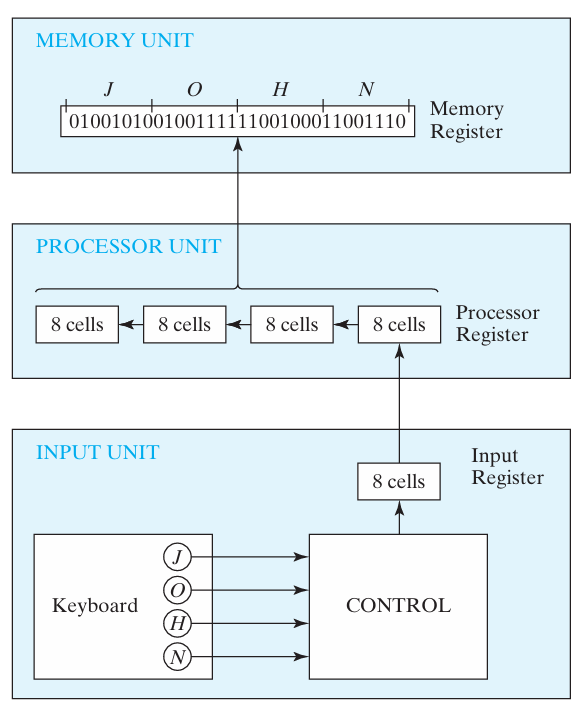
\includegraphics[width=0.9\textwidth]{figs/figure1.png}
    \caption{transfer of information among registers}
    \label{fig:enter-label}
\end{figure}

The image given below shows how a computer stores typed letters in memory. When you press a key, it turns into an 8-bit code and goes into a small storage (input register). Then, it moves to another storage (processor register) and finally gets saved in memory. This process happens for each letter, one by one. Registers help store and move data inside a computer.

\newpage
To process discrete quantities of information in binary form, a computer must be 
provided with devices that hold the data to be processed and with circuit elements that 
manipulate individual bits of information.\textbf{ The device most commonly used for holding 
data is a register.}
Binary variables are manipulated by means of digital logic circuits.

As in above figure, The memory unit has many registers for storing data, while the processor unit has three registers (R1, R2, and R3) and logic circuits for processing. Memory registers store data but cannot perform calculations. Data from memory is moved to processor registers (R1 and R2), where logic circuits add them and store the result in R3. The result can then be sent back to memory for later use. 
\begin{figure}
    \centering
    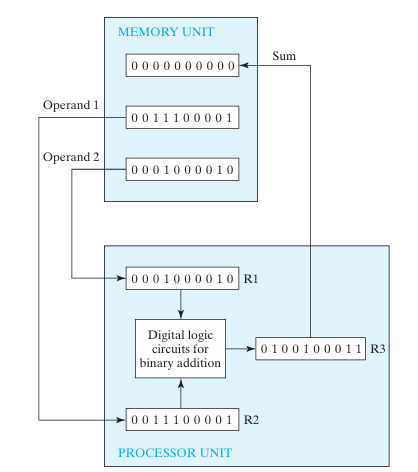
\includegraphics[width=0.926\textwidth]{figs/figure2.png}
    \caption{Example of registers in binary information processing}
    \label{fig:enter-label}
\end{figure}
The registers of the system are the basic elements for storing and 
holding the binary information. 
\end{document}
